
%% bare_jrnl_compsoc.tex
%% V1.3
%% 2007/01/11
%% by Michael Shell
%% See:
%% http://www.michaelshell.org/
%% for current contact information.
%%
%% This is a skeleton file demonstrating the use of IEEEtran.cls
%% (requires IEEEtran.cls version 1.7 or later) with an IEEE Computer
%% Society journal paper.
%%
%% Support sites:
%% http://www.michaelshell.org/tex/ieeetran/
%% http://www.ctan.org/tex-archive/macros/latex/contrib/IEEEtran/
%% andbgf
%% http://www.ieee.org/

%%*************************************************************************
%% Legal Notice:
%% This code is offered as-is without any warranty either expressed or
%% implied; without even the implied warranty of MERCHANTABILITY or
%% FITNESS FOR A PARTICULAR PURPOSE! 
%% User assumes all risk.
%% In no event shall IEEE or any contributor to this code be liable for
%% any damages or losses, including, but not limited to, incidental,
%% consequential, or any other damages, resulting from the use or misuse
%% of any information contained here.
%%
%% All comments are the opinions of their respective authors and are not
%% necessarily endorsed by the IEEE.
%%
%% This work is distributed under the LaTeX Project Public License (LPPL)
%% ( http://www.latex-project.org/ ) version 1.3, and may be freely used,
%% distributed and modified. A copy of the LPPL, version 1.3, is included
%% in the base LaTeX documentation of all distributions of LaTeX released
%% 2003/12/01 or later.
%% Retain all contribution notices and credits.
%% ** Modified files should be clearly indicated as such, including  **
%% ** renaming them and changing author support contact information. **
%%
%% File list of work: IEEEtran.cls, IEEEtran_HOWTO.pdf, bare_adv.tex,
%%                    bare_conf.tex, bare_jrnl.tex, bare_jrnl_compsoc.tex
%%*************************************************************************

% *** Authors should verify (and, if needed, correct) their LaTeX system  ***
% *** with the testflow diagnostic prior to trusting their LaTeX platform ***
% *** with production work. IEEE's font choices can trigger bugs that do  ***
% *** not appear when using other class files.                            ***
% The testflow support page is at:
% http://www.michaelshell.org/tex/testflow/




% Note that the a4paper option is mainly intended so that authors in
% countries using A4 can easily print to A4 and see how their papers will
% look in print - the typesetting of the document will not typically be
% affected with changes in paper size (but the bottom and side margins will).
% Use the testflow package mentioned above to verify correct handling of
% both paper sizes by the user's LaTeX system.
%
% Also note that the "draftcls" or "draftclsnofoot", not "draft", option
% should be used if it is desired that the figures are to be displayed in
% draft mode.
%
% The Computer Society usually requires 10pt for submissions.
%
\documentclass[10pt,journal,cspaper,compsoc]{IEEEtran}
%
% If IEEEtran.cls has not been installed into the LaTeX system files,
% manually specify the path to it like:
% \documentclass[12pt,journal,compsoc]{../sty/IEEEtran}





% Some very useful LaTeX packages include:
% (uncomment the ones you want to load)


% *** MISC UTILITY PACKAGES ***
%
%\usepackage{ifpdf}
% Heiko Oberdiek's ifpdf.sty is very useful if you need conditional
% compilation based on whether the output is pdf or dvi.
% usage:
% \ifpdf
%   % pdf code
% \else
%   % dvi code
% \fi
% The latest version of ifpdf.sty can be obtained from:
% http://www.ctan.org/tex-archive/macros/latex/contrib/oberdiek/
% Also, note that IEEEtran.cls V1.7 and later provides a builtin
% \ifCLASSINFOpdf conditional that works the same way.
% When switching from latex to pdflatex and vice-versa, the compiler may
% have to be run twice to clear warning/error messages.






% *** CITATION PACKAGES ***
%
\ifCLASSOPTIONcompsoc
  % IEEE Computer Society needs nocompress option
  % requires cite.sty v4.0 or later (November 2003)
  % \usepackage[nocompress]{cite}
\else
  % normal IEEE
  % \usepackage{cite}
\fi
% cite.sty was written by Donald Arseneau
% V1.6 and later of IEEEtran pre-defines the format of the cite.sty package
% \cite{} output to follow that of IEEE. Loading the cite package will
% result in citation numbers being automatically sorted and properly
% "compressed/ranged". e.g., [1], [9], [2], [7], [5], [6] without using
% cite.sty will become [1], [2], [5]--[7], [9] using cite.sty. cite.sty's
% \cite will automatically add leading space, if needed. Use cite.sty's
% noadjust option (cite.sty V3.8 and later) if you want to turn this off.
% cite.sty is already installed on most LaTeX systems. Be sure and use
% version 4.0 (2003-05-27) and later if using hyperref.sty. cite.sty does
% not currently provide for hyperlinked citations.
% The latest version can be obtained at:
% http://www.ctan.org/tex-archive/macros/latex/contrib/cite/
% The documentation is contained in the cite.sty file itself.
%
% Note that some packages require special options to format as the Computer
% Society requires. In particular, Computer Society  papers do not use
% compressed citation ranges as is done in typical IEEE papers
% (e.g., [1]-[4]). Instead, they list every citation separately in order
% (e.g., [1], [2], [3], [4]). To get the latter we need to load the cite
% package with the nocompress option which is supported by cite.sty v4.0
% and later. Note also the use of a CLASSOPTION conditional provided by
% IEEEtran.cls V1.7 and later.





% *** GRAPHICS RELATED PACKAGES ***
%
\ifCLASSINFOpdf
  \usepackage[pdftex]{graphicx}
  % declare the path(s) where your graphic files are
  % \graphicspath{{../pdf/}{../jpeg/}}
  % and their extensions so you won't have to specify these with
  % every instance of \includegraphics
  % \DeclareGraphicsExtensions{.pdf,.jpeg,.png}
\else
  % or other class option (dvipsone, dvipdf, if not using dvips). graphicx
  % will default to the driver specified in the system graphics.cfg if no
  % driver is specified.
  \usepackage[dvips]{graphicx}
  % declare the path(s) where your graphic files are
  % \graphicspath{{../eps/}}
  % and their extensions so you won't have to specify these with
  % every instance of \includegraphics
  % \DeclareGraphicsExtensions{.eps}
\fi
% graphicx was written by David Carlisle and Sebastian Rahtz. It is
% required if you want graphics, photos, etc. graphicx.sty is already
% installed on most LaTeX systems. The latest version and documentation can
% be obtained at: 
% http://www.ctan.org/tex-archive/macros/latex/required/graphics/
% Another good source of documentation is "Using Imported Graphics in
% LaTeX2e" by Keith Reckdahl which can be found as epslatex.ps or
% epslatex.pdf at: http://www.ctan.org/tex-archive/info/
%
% latex, and pdflatex in dvi mode, support graphics in encapsulated
% postscript (.eps) format. pdflatex in pdf mode supports graphics
% in .pdf, .jpeg, .png and .mps (metapost) formats. Users should ensure
% that all non-photo figures use a vector format (.eps, .pdf, .mps) and
% not a bitmapped formats (.jpeg, .png). IEEE frowns on bitmapped formats
% which can result in "jaggedy"/blurry rendering of lines and letters as
% well as large increases in file sizes.
%
% You can find documentation about the pdfTeX application at:
% http://www.tug.org/applications/pdftex

\usepackage{amsfonts}
\usepackage{amssymb,amsmath}

% *** MATH PACKAGES ***
%
%\usepackage[cmex10]{amsmath}
% A popular package from the American Mathematical Society that provides
% many useful and powerful commands for dealing with mathematics. If using
% it, be sure to load this package with the cmex10 option to ensure that
% only type 1 fonts will utilized at all point sizes. Without this option,
% it is possible that some math symbols, particularly those within
% footnotes, will be rendered in bitmap form which will result in a
% document that can not be IEEE Xplore compliant!
%
% Also, note that the amsmath package sets \interdisplaylinepenalty to 10000
% thus preventing page breaks from occurring within multiline equations. Use:
%\interdisplaylinepenalty=2500
% after loading amsmath to restore such page breaks as IEEEtran.cls normally
% does. amsmath.sty is already installed on most LaTeX systems. The latest
% version and documentation can be obtained at:
% http://www.ctan.org/tex-archive/macros/latex/required/amslatex/math/





% *** SPECIALIZED LIST PACKAGES ***
%
%\usepackage{algorithmic}
% algorithmic.sty was written by Peter Williams and Rogerio Brito.
% This package provides an algorithmic environment fo describing algorithms.
% You can use the algorithmic environment in-text or within a figure
% environment to provide for a floating algorithm. Do NOT use the algorithm
% floating environment provided by algorithm.sty (by the same authors) or
% algorithm2e.sty (by Christophe Fiorio) as IEEE does not use dedicated
% algorithm float types and packages that provide these will not provide
% correct IEEE style captions. The latest version and documentation of
% algorithmic.sty can be obtained at:
% http://www.ctan.org/tex-archive/macros/latex/contrib/algorithms/
% There is also a support site at:
% http://algorithms.berlios.de/index.html
% Also of interest may be the (relatively newer and more customizable)
% algorithmicx.sty package by Szasz Janos:
% http://www.ctan.org/tex-archive/macros/latex/contrib/algorithmicx/




% *** ALIGNMENT PACKAGES ***
%
%\usepackage{array}
% Frank Mittelbach's and David Carlisle's array.sty patches and improves
% the standard LaTeX2e array and tabular environments to provide better
% appearance and additional user controls. As the default LaTeX2e table
% generation code is lacking to the point of almost being broken with
% respect to the quality of the end results, all users are strongly
% advised to use an enhanced (at the very least that provided by array.sty)
% set of table tools. array.sty is already installed on most systems. The
% latest version and documentation can be obtained at:
% http://www.ctan.org/tex-archive/macros/latex/required/tools/


%\usepackage{mdwmath}
%\usepackage{mdwtab}
% Also highly recommended is Mark Wooding's extremely powerful MDW tools,
% especially mdwmath.sty and mdwtab.sty which are used to format equations
% and tables, respectively. The MDWtools set is already installed on most
% LaTeX systems. The lastest version and documentation is available at:
% http://www.ctan.org/tex-archive/macros/latex/contrib/mdwtools/


% IEEEtran contains the IEEEeqnarray family of commands that can be used to
% generate multiline equations as well as matrices, tables, etc., of high
% quality.


%\usepackage{eqparbox}
% Also of notable interest is Scott Pakin's eqparbox package for creating
% (automatically sized) equal width boxes - aka "natural width parboxes".
% Available at:
% http://www.ctan.org/tex-archive/macros/latex/contrib/eqparbox/





% *** SUBFIGURE PACKAGES ***
%\ifCLASSOPTIONcompsoc
%\usepackage[tight,normalsize,sf,SF]{subfigure}
%\else
%\usepackage[tight,footnotesize]{subfigure}
%\fi
% subfigure.sty was written by Steven Douglas Cochran. This package makes it
% easy to put subfigures in your figures. e.g., "Figure 1a and 1b". For IEEE
% work, it is a good idea to load it with the tight package option to reduce
% the amount of white space around the subfigures. Computer Society papers
% use a larger font and \sffamily font for their captions, hence the
% additional options needed under compsoc mode. subfigure.sty is already
% installed on most LaTeX systems. The latest version and documentation can
% be obtained at:
% http://www.ctan.org/tex-archive/obsolete/macros/latex/contrib/subfigure/
% subfigure.sty has been superceeded by subfig.sty.


%\ifCLASSOPTIONcompsoc
%  \usepackage[caption=false]{caption}
%  \usepackage[font=normalsize,labelfont=sf,textfont=sf]{subfig}
%\else
%  \usepackage[caption=false]{caption}
%  \usepackage[font=footnotesize]{subfig}
%\fi
% subfig.sty, also written by Steven Douglas Cochran, is the modern
% replacement for subfigure.sty. However, subfig.sty requires and
% automatically loads Axel Sommerfeldt's caption.sty which will override
% IEEEtran.cls handling of captions and this will result in nonIEEE style
% figure/table captions. To prevent this problem, be sure and preload
% caption.sty with its "caption=false" package option. This is will preserve
% IEEEtran.cls handing of captions. Version 1.3 (2005/06/28) and later 
% (recommended due to many improvements over 1.2) of subfig.sty supports
% the caption=false option directly:
%\ifCLASSOPTIONcompsoc
%  \usepackage[caption=false,font=normalsize,labelfont=sf,textfont=sf]{subfig}
%\else
%  \usepackage[caption=false,font=footnotesize]{subfig}
%\fi
%
% The latest version and documentation can be obtained at:
% http://www.ctan.org/tex-archive/macros/latex/contrib/subfig/
% The latest version and documentation of caption.sty can be obtained at:
% http://www.ctan.org/tex-archive/macros/latex/contrib/caption/




% *** FLOAT PACKAGES ***
%
%\usepackage{fixltx2e}
% fixltx2e, the successor to the earlier fix2col.sty, was written by
% Frank Mittelbach and David Carlisle. This package corrects a few problems
% in the LaTeX2e kernel, the most notable of which is that in current
% LaTeX2e releases, the ordering of single and double column floats is not
% guaranteed to be preserved. Thus, an unpatched LaTeX2e can allow a
% single column figure to be placed prior to an earlier double column
% figure. The latest version and documentation can be found at:
% http://www.ctan.org/tex-archive/macros/latex/base/



%\usepackage{stfloats}
% stfloats.sty was written by Sigitas Tolusis. This package gives LaTeX2e
% the ability to do double column floats at the bottom of the page as well
% as the top. (e.g., "\begin{figure*}[!b]" is not normally possible in
% LaTeX2e). It also provides a command:
%\fnbelowfloat
% to enable the placement of footnotes below bottom floats (the standard
% LaTeX2e kernel puts them above bottom floats). This is an invasive package
% which rewrites many portions of the LaTeX2e float routines. It may not work
% with other packages that modify the LaTeX2e float routines. The latest
% version and documentation can be obtained at:
% http://www.ctan.org/tex-archive/macros/latex/contrib/sttools/
% Documentation is contained in the stfloats.sty comments as well as in the
% presfull.pdf file. Do not use the stfloats baselinefloat ability as IEEE
% does not allow \baselineskip to stretch. Authors submitting work to the
% IEEE should note that IEEE rarely uses double column equations and
% that authors should try to avoid such use. Do not be tempted to use the
% cuted.sty or midfloat.sty packages (also by Sigitas Tolusis) as IEEE does
% not format its papers in such ways.




%\ifCLASSOPTIONcaptionsoff
%  \usepackage[nomarkers]{endfloat}
% \let\MYoriglatexcaption\caption
% \renewcommand{\caption}[2][\relax]{\MYoriglatexcaption[#2]{#2}}
%\fi
% endfloat.sty was written by James Darrell McCauley and Jeff Goldberg.
% This package may be useful when used in conjunction with IEEEtran.cls'
% captionsoff option. Some IEEE journals/societies require that submissions
% have lists of figures/tables at the end of the paper and that
% figures/tables without any captions are placed on a page by themselves at
% the end of the document. If needed, the draftcls IEEEtran class option or
% \CLASSINPUTbaselinestretch interface can be used to increase the line
% spacing as well. Be sure and use the nomarkers option of endfloat to
% prevent endfloat from "marking" where the figures would have been placed
% in the text. The two hack lines of code above are a slight modification of
% that suggested by in the endfloat docs (section 8.3.1) to ensure that
% the full captions always appear in the list of figures/tables - even if
% the user used the short optional argument of \caption[]{}.
% IEEE papers do not typically make use of \caption[]'s optional argument,
% so this should not be an issue. A similar trick can be used to disable
% captions of packages such as subfig.sty that lack options to turn off
% the subcaptions:
% For subfig.sty:
% \let\MYorigsubfloat\subfloat
% \renewcommand{\subfloat}[2][\relax]{\MYorigsubfloat[]{#2}}
% For subfigure.sty:
% \let\MYorigsubfigure\subfigure
% \renewcommand{\subfigure}[2][\relax]{\MYorigsubfigure[]{#2}}
% However, the above trick will not work if both optional arguments of
% the \subfloat/subfig command are used. Furthermore, there needs to be a
% description of each subfigure *somewhere* and endfloat does not add
% subfigure captions to its list of figures. Thus, the best approach is to
% avoid the use of subfigure captions (many IEEE journals avoid them anyway)
% and instead reference/explain all the subfigures within the main caption.
% The latest version of endfloat.sty and its documentation can obtained at:
% http://www.ctan.org/tex-archive/macros/latex/contrib/endfloat/
%
% The IEEEtran \ifCLASSOPTIONcaptionsoff conditional can also be used
% later in the document, say, to conditionally put the References on a 
% page by themselves.




% *** PDF, URL AND HYPERLINK PACKAGES ***
%
%\usepackage{url}
% url.sty was written by Donald Arseneau. It provides better support for
% handling and breaking URLs. url.sty is already installed on most LaTeX
% systems. The latest version can be obtained at:
% http://www.ctan.org/tex-archive/macros/latex/contrib/misc/
% Read the url.sty source comments for usage information. Basically,
% \url{my_url_here}.





% *** Do not adjust lengths that control margins, column widths, etc. ***
% *** Do not use packages that alter fonts (such as pslatex).         ***
% There should be no need to do such things with IEEEtran.cls V1.6 and later.
% (Unless specifically asked to do so by the journal or conference you plan
% to submit to, of course. )


% correct bad hyphenation here
\hyphenation{op-tical net-works semi-conduc-tor}


\begin{document}
%
% paper title
% can use linebreaks \\ within to get better formatting as desired
\title{Efficient Coalition Formation \\ for Web Services}
%
%
% author names and IEEE memberships
% note positions of commas and nonbreaking spaces ( ~ ) LaTeX will not break
% a structure at a ~ so this keeps an author's name from being broken across
% two lines.
% use \thanks{} to gain access to the first footnote area
% a separate \thanks must be used for each paragraph as LaTeX2e's \thanks
% was not built to handle multiple paragraphs
%
%
%\IEEEcompsocitemizethanks is a special \thanks that produces the bulleted
% lists the Computer Society journals use for "first footnote" author
% affiliations. Use \IEEEcompsocthanksitem which works much like \item
% for each affiliation group. When not in compsoc mode,
% \IEEEcompsocitemizethanks becomes like \thanks and
% \IEEEcompsocthanksitem becomes a line break with idention. This
% facilitates dual compilation, although admittedly the differences in the
% desired content of \author between the different types of papers makes a
% one-size-fits-all approach a daunting prospect. For instance, compsoc 
% journal papers have the author affiliations above the "Manuscript
% received ..."  text while in non-compsoc journals this is reversed. Sigh.

\author{Michael~Shell,~\IEEEmembership{Member,~IEEE,}
        John~Doe,~\IEEEmembership{Fellow,~OSA,}
        and~Jane~Doe,~\IEEEmembership{Life~Fellow,~IEEE}% <-this % stops a space
\IEEEcompsocitemizethanks{\IEEEcompsocthanksitem M. Shell is with the Department
of Electrical and Computer Engineering, Georgia Institute of Technology, Atlanta,
GA, 30332.\protect\\
% note need leading \protect in front of \\ to get a newline within \thanks as
% \\ is fragile and will error, could use \hfil\break instead.
E-mail: see http://www.michaelshell.org/contact.html
\IEEEcompsocthanksitem J. Doe and J. Doe are with Anonymous University.}% <-this % stops a space
\thanks{}}

% note the % following the last \IEEEmembership and also \thanks - 
% these prevent an unwanted space from occurring between the last author name
% and the end of the author line. i.e., if you had this:
% 
% \author{....lastname \thanks{...} \thanks{...} }
%                     ^------------^------------^----Do not want these spaces!
%
% a space would be appended to the last name and could cause every name on that
% line to be shifted left slightly. This is one of those "LaTeX things". For
% instance, "\textbf{A} \textbf{B}" will typeset as "A B" not "AB". To get
% "AB" then you have to do: "\textbf{A}\textbf{B}"
% \thanks is no different in this regard, so shield the last } of each \thanks
% that ends a line with a % and do not let a space in before the next \thanks.
% Spaces after \IEEEmembership other than the last one are OK (and needed) as
% you are supposed to have spaces between the names. For what it is worth,
% this is a minor point as most people would not even notice if the said evil
% space somehow managed to creep in.



% The paper headers
\markboth{Journal of \LaTeX\ Class Files,~Vol.~6, No.~1, January~2007}%
{Shell \MakeLowercase{\textit{et al.}}: Bare Demo of IEEEtran.cls for Computer Society Journals}
% The only time the second header will appear is for the odd numbered pages
% after the title page when using the twoside option.
% 
% *** Note that you probably will NOT want to include the author's ***
% *** name in the headers of peer review papers.                   ***
% You can use \ifCLASSOPTIONpeerreview for conditional compilation here if
% you desire.



% The publisher's ID mark at the bottom of the page is less important with
% Computer Society journal papers as those publications place the marks
% outside of the main text columns and, therefore, unlike regular IEEE
% journals, the available text space is not reduced by their presence.
% If you want to put a publisher's ID mark on the page you can do it like
% this:
%\IEEEpubid{0000--0000/00\$00.00~\copyright~2007 IEEE}
% or like this to get the Computer Society new two part style.
%\IEEEpubid{\makebox[\columnwidth]{\hfill 0000--0000/00/\$00.00~\copyright~2007 IEEE}%
%\hspace{\columnsep}\makebox[\columnwidth]{Published by the IEEE Computer Society\hfill}}
% Remember, if you use this you must call \IEEEpubidadjcol in the second
% column for its text to clear the IEEEpubid mark (Computer Society jorunal
% papers don't need this extra clearance.)




% for Computer Society papers, we must declare the abstract and index terms
% PRIOR to the title within the \IEEEcompsoctitleabstractindextext IEEEtran
% command as these need to go into the title area created by \maketitle.
\IEEEcompsoctitleabstractindextext{%
\begin{abstract}
%\boldmath
Web services are loosely-coupled business applications willing to
cooperate in distributed settings within different groups called
communities. Communities aim to provide better visibility,
efficiency, market share and total payoff. There are a number of
proposed mechanisms and models on aggregating web services and
making them cooperate within their communities. However, forming
optimal and stable communities as coalitions to maximize
individual and group efficiency and income has not been addressed
yet. In this paper, we propose an efficient coalition formation
mechanism using cooperative game-theoretic techniques. We propose
a mechanism for community membership requests and selections of
web services in the scenarios where established communities
already exist. Moreover, we analyze the scenarios where
communities are not established yet and web services can form multiple communities. The ultimate objective is to
develop a mechanism for web services to form stable groups
allowing them to maximize their efficiency and generate
near-optimal (welfare-maximizing) communities. The theoretical and
simulation results show that our algorithms provide web services
and community owners with applicable and near-optimal decision
making mechanisms.
\end{abstract}
% IEEEtran.cls defaults to using nonbold math in the Abstract.
% This preserves the distinction between vectors and scalars. However,
% if the journal you are submitting to favors bold math in the abstract,
% then you can use LaTeX's standard command \boldmath at the very start
% of the abstract to achieve this. Many IEEE journals frown on math
% in the abstract anyway. In particular, the Computer Society does
% not want either math or citations to appear in the abstract.

% Note that keywords are not normally used for peer review papers.
\begin{keywords}
Web services; Cooperative game theory; Community of services;
\end{keywords}}


% make the title area
\maketitle


% To allow for easy dual compilation without having to reenter the
% abstract/keywords data, the \IEEEcompsoctitleabstractindextext text will
% not be used in maketitle, but will appear (i.e., to be "transported")
% here as \IEEEdisplaynotcompsoctitleabstractindextext when compsoc mode
% is not selected <OR> if conference mode is selected - because compsoc
% conference papers position the abstract like regular (non-compsoc)
% papers do!
\IEEEdisplaynotcompsoctitleabstractindextext
% \IEEEdisplaynotcompsoctitleabstractindextext has no effect when using
% compsoc under a non-conference mode.


% For peer review papers, you can put extra information on the cover
% page as needed:
% \ifCLASSOPTIONpeerreview
% \begin{center} \bfseries EDICS Category: 3-BBND \end{center}
% \fi
%
% For peerreview papers, this IEEEtran command inserts a page break and
% creates the second title. It will be ignored for other modes.
\IEEEpeerreviewmaketitle



\section{Introduction}

\IEEEPARstart{O}{ver} the past years, online services have become part of many
scalable business applications. The increasing reliance on
web-based applications has significantly influenced the way web
services are engineered. Web services provide a set of stateless
software functions accessible at a network address over the web.
The recent developments are shifting web services from passive and
individual components to autonomous and group-based components
where interaction, composition, and cooperation are the key
challenges \cite{ICWS2011-1,SCC2011-1}. The main objective is to
achieve a seamless integration of business processes, applications
and web services. Delivering high quality services considering the
dynamic and unpredictable nature of the Internet is still a very
critical and challenging issue.

The need for highly available and responsive services has called
for grouping and collaborative mechanisms of loosely-coupled web
services, particularly in business settings. The idea of grouping
web services within communities and the way those communities are
engineered so that web services can better collaborate have been
proposed and investigated in
\cite{DBLP:journals/ijebr/MaamarSTBB09,DBLP:journals/internet/BenatallahSD03,Rosario:2008:PQS:1512146.1512290}.
Communities are virtual groups of web services having similar
functionalities, but probably different non-functional quality
attributes, which form the QoS parameters. When communities are
used, users send their requests to the masters of those
communities, which are responsible of managing the communities,
forwarding the requests to the suitable member web services and
checking the credentials of those members. Communities aim to
provide higher service availability and performance than what
individual web services can provide. The high availability of
services and the community resilience to failure are guaranteed
since web services can cooperate and replace each other within the
same community and since there is no single point of failure in
the communities architecture.

Most of the recent work on communities of services are either
user-centric and focus on user satisfaction
\cite{Chun02user-centricperformance} or system-centric and focus
on the whole system throughput, performance and utilization. There
are many contributions in distributed, grid, cluster and cloud
services which are system-centric. However, in real world
environments and applications, both users and service providers
are self-interested agents, aiming to maximize their own profit.
In those environments, both parties (users and services) will
collaborate as long as they are getting more benefits and payoff.

In this direction, recently \cite{DBLP:conf/IEEEscc/LimTMB12,
DBLP:conf/IEEEscc/KhosravifarABT11} proposed mechanisms to help
users and services maximize their gain. A two-player
non-cooperative game between web services and community master was
introduced in \cite{DBLP:conf/IEEEscc/KhosravifarABT11}. In this
game-theoretic model, the strategies available to a web service
when facing a new community are requesting to join the community,
accepting the master's invitation to join the community, or
refusing the invitation to join. The set of strategies for
communities are inviting the web service or refusing the web
service's join request. Based on their capacity, market share and
reputation, the two players have different set of utilities over
the strategy profiles of the game. The main limits of this game
model are: 1) its consideration of only three quality parameters,
while the other factors are simply ignored; and 2) the
non-consideration of the web services already residing within the
community. The game is only between the community master and the
new web service, and the inputs from all the other members are
simply ignored. The consideration of those inputs is a significant
issue as existing web services can lose utility or payoff because
of the new member, which can results in an unhealthy and unstable
group. The problem comes from the fact that the existing members
should collaborate with the new web services, so probably their
performance as a group can suffer. Existing members may even
deviate and try to join other communities if they are unsatisfied.
Those considerations of forming stable and efficient coalitions
are the main contributions of our paper.

In \cite{DBLP:conf/IEEEscc/LimTMB12} a 3-way satisfaction approach
for selecting web services has been proposed. In this approach,
the authors proposed a web service selection process that the
community masters can use. The approach considerers the efficiency
of all the three involved parties, namely users, web services and
communities. In this work, it is shown how the gains of these
parties are coupled together using a linear optimization process.
However, the optimization problem in this solution tends to
optimize some parameters considering all web services regardless
of their efficiency and contribution to the community's welfare.
Moreover, there are no clear thresholds for accepting or rejecting
new web services. The solution of the optimization problem could,
for instance, suggest web services already residing within the
community to increase or decrease their capacity to cover up the
weakness of other parties in the system. However, a high
performing web service could deviate anytime it finds itself
unsatisfied within the community instead of adjusting its service
parameters.

\textbf{Contributions.} In this paper, we use game theory to
propose a cooperative game model for the aggregation of web
services within communities. The solution concepts of our
cooperative game seeks to find efficient ways of forming
coalitions (teams) of web services so that they can maximize their
gain and payoff, and distribute the gain in a fair way among all
the web services. Achieving Fairness when the gain is distributed
among the community members is the main factor to keep the
coalition stable as no web service will expect to gain better by
deviating for the community. In other words, the coalition is made
efficient if all the members are satisfied. We first propose a
representation function for communities of web services based on
their QoS attributes. By using this function, we can evaluate the
$worth$ of each community of web services. When facing new
membership requests, a typical community master checks whether the
new coalition having the old and new set of web services will keep
the community stable or not. The community master will reject the
membership requests if it finds out that the new coalition would
be unstable, preventing $any$ subset of web services from gaining
significantly more by deviating from the community and joining
other communities or forming new ones. The computation of
solutions for cooperative game theory problems is combinatorial in
nature and proven to be NP-complete \cite{Algorithmic}, making
this computation impractical in real world applications. However,
using the concepts of coalition stability, we propose
approximation algorithms running in polynomial time providing web
services and community masters with applicable and near-optimal
decision making mechanisms.

The rest of paper is organized as follows. Section
\ref{s:preliminaries} describes the architecture, considered
parameters and some basic cooperative game theory concepts.
Section \ref{s:model} presents our solution model in three
different scenarios. Section \ref{s:resutls} describes our
experiments and results. Finally, Section \ref{s:conclusion},
concludes the paper and identifies future work.

% Computer Society journal papers do something a tad strange with the very
% first section heading (almost always called "Introduction"). They place it
% ABOVE the main text! IEEEtran.cls currently does not do this for you.
% However, You can achieve this effect by making LaTeX jump through some
% hoops via something like:
%
%\ifCLASSOPTIONcompsoc
%  \noindent\raisebox{2\baselineskip}[0pt][0pt]%
%  {\parbox{\columnwidth}{\section{Introduction}\label{sec:introduction}%
%  \global\everypar=\everypar}}%
%  \vspace{-1\baselineskip}\vspace{-\parskip}\par
%\else
%  \section{Introduction}\label{sec:introduction}\par
%\fi
%
% Admittedly, this is a hack and may well be fragile, but seems to do the
% trick for me. Note the need to keep any \label that may be used right
% after \section in the above as the hack puts \section within a raised box.



% The very first letter is a 2 line initial drop letter followed
% by the rest of the first word in caps (small caps for compsoc).
% 
% form to use if the first word consists of a single letter:
% \IEEEPARstart{A}{demo} file is ....
% 
% form to use if you need the single drop letter followed by
% normal text (unknown if ever used by IEEE):
% \IEEEPARstart{A}{}demo file is ....
% 
% Some journals put the first two words in caps:
% \IEEEPARstart{T}{his demo} file is ....
% 
% Here we have the typical use of a "T" for an initial drop letter
% and "HIS" in caps to complete the first word.
%\IEEEPARstart{T}{his} demo file is intended to serve as a ``starter file''
%for IEEE Computer Society journal papers produced under \LaTeX\ using
%IEEEtran.cls version 1.7 and later.
% You must have at least 2 lines in the paragraph with the drop letter
% (should never be an issue)
%I wish you the best of success.

%\hfill mds
 
%\hfill January 11, 2007


\section{Preliminaries}\label{s:preliminaries}

In this section, we discuss the parameters and preliminary
concepts that we use in the rest of the paper.

\subsection{The Architecture}

Our system consists of three main types of entities working
together:

\emph{1) Web services} are rational entities\footnote{The term
rational is used here in the sense that web services are utility
maximizers} providing services to end users. They aim to maximize
their individual income by receiving enough requests from end
users. In order to increase their revenue, web services seek for
more tasks if they have the capacity and throughput to do so. Web
services can join communities to have better efficiency by
collaborating with others, to have access to higher market share,
and to have opportunity of receiving a bigger task pool from end
users. Throughout this paper, in
our equations, we refer to web services as $ws$ and to the set of
web services hosted by a given community as $C$. To simply the
notation, sometimes we simply write $ws$ instead of $ws \in C$ to
go through the elements $ws$ of the set $C$.

\emph{2) Master Web Services} or the community coordinators, are representatives of the
communities of web services and responsible for their management.
Communities receive requests from users and aim to host a healthy
set of web services to perform the required tasks. They seek to
maximize user satisfaction by having tasks accomplished according
to the desired QoS. In fact, higher user satisfaction will bring
more user requests and increase the market share and revenue of
the community.

\emph{3) Users} generate requests and try to find the best
available services. User satisfaction is abstracted as function of
quantity and quality of tasks accomplished by a given service.

\subsection{Web Service Parameters}\label{ws_parameters}

Web services come with different quality of service parameters.
These parameters with a short description are listed in Table
\ref{qosws}.

\begin{table}[!t]
\centering
\caption{List of web service QoS parameters.}
\begin{tabular}{|c|c||c|c|}
\hline
\textbf{Parameter} & \textbf{Definition} \\
\hline\hline
$Availability$ & Probability of being available during \\
&a time frame \\
$Reliability$ & Probability of successfully handling \\
&requests during a timeframe\\
$Successability$ & Rate of successfully handled requests \\
$Throughput$ & Average rate of handling requests \\
$Latency$ & The average latency of services\\
$Capacity$ & Amount of resources available\\
$Cost$ & Mean service fee \\
$Regulatory$ & Compliance with standards, law and rules\\
$Security$ & Quality of confidentiality \\ 
&and non-repudiation\\
\hline
\end{tabular}
\label{qosws}
\end{table}

We adopted a real world dataset \cite{DBLP:conf/smc/Al-MasriM09a}
which has aggregated and normalized each of these parameters to a
real value between 0 and 1. Since requests are not shared among
web services and are distributed among all of them inside a
community, each one of them comes with a given QoS denoted by
$(QoS_{ws})$. We assume that $(QoS_{ws})$ is obtained by a certain
aggregation function of the parameters considered in Table
\ref{qosws}. We use this quality output later in evaluating the
community \emph{worth} or \emph{payoff} function.

\subsection{Web Service Communities}\label{webservice-communities}

Figure \ref{fig_community} represents the architecture of web service communities. The communities are basicly an abstract model of web services, they aggrigate web services and communicate with other entities such as UDDI registeries and users, using identical protocols as web services. Web services join communities to increase their utility by having a larger market share and task pool. Community cordinators or master web services are responsible for community development, managing membership requests from web services and distributing user tasks among the community members. Communitiy coordinators try to attract quality web services and keep the community as stable and productive as possible to gain better reputation and user satisfaction which results in having a higher market share for the community. The way the web services reside inside communities and how communities of web services are engineered is described comprehensivly in \cite{DBLP:journals/ijebr/MaamarSTBB09}.

\begin{figure*}[!t]
\centerline{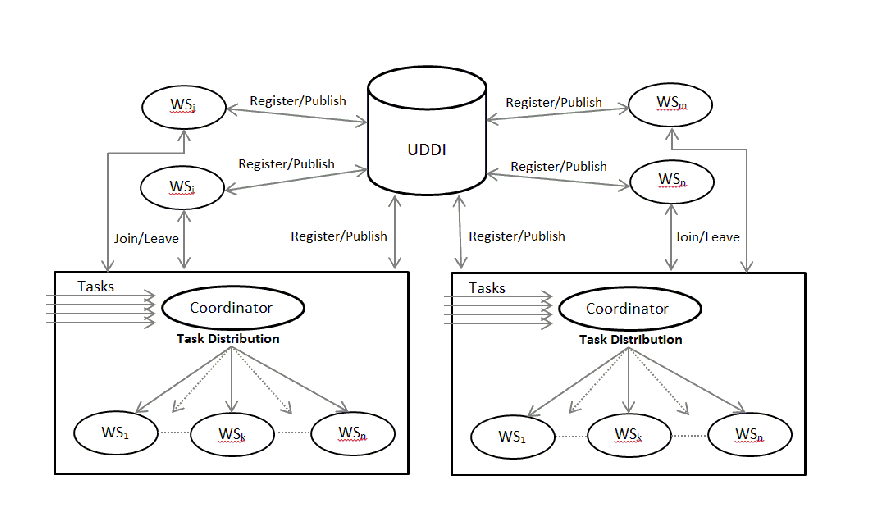
\includegraphics[width=6.25in]{community.eps}}
\caption{Architecture of Web Service communities}
\label{fig_community}
\end{figure*}

\subsection{Cooperative Game Concepts}
Cooperative game is a branch of game theory that studies
strategies of self-interested entities or agents in a setting
where those agents can increase their payoff by binding agreements
and cooperating in groups. We let $N$ be a set of players. Any
subset $S$ of $N$ can form a group called $coalition$. A
\emph{coalitional game} is a pair $G = (N, v)$ where $v$ is called
a \emph{characteristic function}, which given a coalition, is a
function $v: 2^N \to \mathbb{R}$ mapping the set of players of the
coalition to a real number $v(S)$, the worth of $S$. This number
usually represents the output or payoff or again the performance
of these players working together as coalition.  If a coalition
$S$ is formed, then it can divide its worth, $v(S)$ in any
possible way among its members. The payoff vector $x \in
\mathbb{R}^S$ is the amount of payoff being distributed among the
members of the coalition $S$. The payoff vector satisfies two
conditions:

\begin{itemize}
    \item $x_i \geq 0$ for all $i \in N$, and
    \item $\sum_{i \in S} x_i \leq v(S)$
\end{itemize}

The second criteria is called the \emph{feasibility} condition,
according to which, the payoff for each agent cannot be more than
the coalition total gain. A payoff vector is also \emph{efficient}
if the payoff obtained by a coalition is distributed amongst the
coalition members: $\sum_{i \in S} x_i = v(S)$. This definition of
the characteristic function works in \emph{transferable utility}
(TU) settings, where utility (i.e., payoff) is transferable from
one player to another, or in other words, players have common
currency and a unit of income is worth same for all players
\cite{myerson1991game}.

When dealing with cooperative games, two issues need to be
addressed:\\ 1. What coalitions to form? \\
2. How to reward each member when a task is completed?\\
%
The following definitions help address these two issues.

%\subsubsection{Shapley value}

{\bf Definition 1 (Shapley value)} Given a cooperative game $(N,
v)$, the \emph{Shapley value} of player $i$ is given
by\cite{shapley_value}:
\begin{equation}\label{eq:shapley}
\phi_i(N,v) = \sum_{S \subseteq N \backslash \left\{i\right\} }
\frac{|S|! (|N|-|S|-1)!}{|N|!} (v(S \cup \left\{i\right\}) - v(S))
\end{equation}

\emph{Shapley value} is a unique and fair solution concept for
payoff distribution among the members of the coalition. It
basically rewards members with the amount of marginal contribution
they have to the coalition.

%\subsubsection{Core}

{\bf Definition 2 (Core)} A payoff vector $x$ is in the $core$ of
a coalitional game $(N, v)$ if and only if:
\begin{equation}\label{eq:core}
\forall S \subseteq N, \sum_{x_i \in S} x_i \geq v(S)
\end{equation}

The core is basically a set of payoff vectors where no subset of
players $S^\prime$ could gain more than their current payoff by
deviating and making their own coalition $\sum_{i \in S^\prime}
x_i \geq v(S^\prime)$. The sum of payoffs of the players in any
sub-coalition $S$ is at least as large as the amount that these
players could earn by forming a coalition by their own. In a
sense, it is analogue to Nash equilibrium, except that core is
about deviations from groups of entities. The core is the
strongest and most popular solution concept in cooperative game
theory. However, its computation is a combinatorial problem and
becomes intractable as the number of players increases. The core
of some real-world problem games may be empty, which means having
the characteristic function of the game $(N,v)$, there might be no
possible distribution of payoff assuring stability of subgroups.

{\bf Definition 3 (Convex cooperative games)} A game $(N,v)$ with
characteristic function $v(S)$ is convex if:
\begin{equation}\label{eq:convex}
v(S) + v(T) \leq v(S \cup T) + v (S \cap T), \forall S,T \subseteq
N.
\end{equation}

According to a classic result by Shapley \cite{S1971cores}, convex
games always have a non-empty core. We will use a variation of
convexity condition in our algorithm to check whether our
coalitions are stable.

\subsubsection*{$\epsilon$-core}\label{s:epsilon}
%\emph{$\epsilon$-Core:}
%\\
When the \emph{core} set of a game is empty, it means no coalition
of players can gain anything by deviating. An outcome would be
unstable if a coalition can benefit even by a small amount from
deviating, which is a strong requirement. In fact, in some
situations, deviations can be costly, or players may have loyalty
to their coalitions, or even it can be computationally intractable
to find those small benefits. It would only make sense for a
coalition to deviate if the gain from a deviation exceeds the cost
of performing the deviation. \emph{$\epsilon$-core} relaxes the
notion of the core, and only requires that no coalition would
benefit significantly, or within a constant amount($\epsilon$) by
deviating (see Equation \ref{eq:core}).

\begin{equation}\label{eq:core2}
\forall S \subseteq N, \sum_{x_i \in S} x_i \geq v(S) - \epsilon
\end{equation}

\subsubsection*{Coalition Structure Formation}\label{sec:coalition}

Coalition structure formation is the problem of finding the best
partition of web services into teams. In these settings, the
performance of an individual service is less important than the
\emph{social welfare} of the whole system, which is the sum of the
values of all teams. Having the game $(N,v)$, a coalition
structure $(CS)$ is \emph{socially optimal} if $CS$ belongs to set
$\operatorname*{arg\,max}_{CS} v(CS)$ where $v(CS)$ is the sum of
the values of all coalitions inside $CS$. $v(CS) = \sum_{C \in
CS}v(C)$.
%The outcome of a characteristic function game in coalition structure settings, consists of two parts; first a disjoint partition of players (agents) into coalitions, called a \emph{coalition structure} (CS) and second a \emph{payoff vector} as mentioned in cooperative game solution concepts, which distributes the value of each coalition among its members.


\section{Problem Formulation and Modeling}\label{s:model}

In this section, we present the web service and community coordinator's intractions, the task distribution process and revenue models in web service communities.

\subsection{Task destribution}

As mentioned in section \ref{webservice-communities}, communities are robust service providers with well stablished market share and reputation. By maintaining their reputation and performance, they attract  end users which choose them as service providers to perform their tasks. The community master is characterizd by a request rate $(R_C)$ from users. Each web service comes with a given QoS ($QoS_{ws}$) from which the throughput $Tr_{ws}$ is excluded. This exclusion allows us to build our analysis on the particular value of $Tr_{ws}$. Throughput is the average rate of tasks a web service can perform per time unit. Thus, web services perform tasks with an average output quality of $QoS_{ws}$ and a throughput rate of $Tr_{ws}$.

The community master uses a slightly modified \emph{weighted fair queuing} method to distribute task among its members. The goal is to allocate incoming tasks to web services with a rate matching throughput value of $Tr_{ws}$. In \emph{weighted fair queuing} method \emph{all} the input flow is multiplexed along different paths, however in our case if the input rate $(R_C)$ of the community is more than summation of throughput values of web services, some of the input tasks will be queued and served with delay. Thus, the amount of tasks performed by community is $\sum_{ws \in C}{(Tr_{ws})}$ when $\sum_{ws}{Tr_{ws}} \leq R_{C}$. However, when the community has more web services having more total throughput value than community's request rate $(R_C)$ the \emph{weighted fair queuing} algorithm assigns a weighted task rate of $R_C \times \frac{Tr_{ws}}{\sum_{ws}{Tr_{ws}}}$ for each web service ($ws$) and the total rate of tasks being performed is $R_C$, the community's receiving request rate.

\subsection{Community Revenue}

The communities and web services earn revenue by performing tasks. The total gain is function of quality ($QoS_{ws}$) and quantity($Tr_{ws}$) of tasks being performed. As mentioned in section \ref{ws_parameters} $QoS_{ws}$ is obtained by a certain aggregation function of the parameters considered in Table \ref{qosws}. We have adopted a linear equal weigth average over all QoS parameteres listed in table \ref{qosws} excluding the $Throuput$ and $Cost$ parameters. A community has the option to weigh specific QoS patameters more or less depending on the expectations of their clients. 

The maximum potential output $(PO(C))$ of a community is aggregation of number of tasks, times their quality, for each web service participating as a member of the community:

\begin{equation}
PO(C) = \sum_{ws \in C}{(T_{ws} \times QoS_{ws})}
\end{equation}

If the summation of throughput ($Tr_{ws}$) values of community members exceeds the input task rate of the community ($R_C$) the community cannot perform at its maximum potential. It means community has more web services than it needs for performing input task load. Therefore, in these cases, the actual output has to be normalized to the ammount of tasks being performed.

\begin{equation}
Out(C) = \left\{
  \begin{array}{l l}
    PO(C) & \quad \text{if $\sum_{ws}{Th_{ws}} \leq R_{M}$}\\
    PO(C) \times \frac{R_{M}}{\sum_{ws}{Th_{ws}}} & \quad \text{if $\sum_{ws}{Th_{ws}} > R_{M}$}
  \end{array} \right.
\end{equation}

The revenue function of the web service community, is a linear function of $Out(C)$ with a positive constant multiplier. 

\subsection{Case Study}

In this section, we analyse a few numerical examples and discuss the motivation of web services and community intractions and the strategies they can adopt and the revenue they can earn adopting different strategies.

%%%%%%%%%%%%%%%%%%%%%%%%% EXAMPLE 1 %%%%%%%%%%%%%%%%%%%%%%%%%%%%%%%%%%%%
\begin{table}[!t]
\renewcommand{\arraystretch}{1.3}
% if using array.sty, it might be a good idea to tweak the value of
% \extrarowheight as needed to properly center the text within the cells
\caption{Three web services of example 1}
\label{example_1}
\centering
\begin{tabular}{c c c c}
\hline
$WS$ & $QoS_{ws}$ & $Th_{ws}$ & $Th_{ws} \times QoS_{ws}$\\
\hline
1 & 0.8 & 4 & 3.2\\
1 & 0.8 & 5 & 4.0\\
1 & 0.8 & 3 & 2.4\\
\hline
\end{tabular}
\end{table}

\begin{table}[!t]
\renewcommand{\arraystretch}{1.3}
% if using array.sty, it might be a good idea to tweak the value of
% \extrarowheight as needed to properly center the text within the cells
% \caption{Three web services}
\label{example_1_1}
\centering
\begin{tabular}{c c || c c}
\hline
Community & Worth & Community & Worth\\
\hline
$\left\{1\right\}$ & 3.2 & $\left\{1,2\right\}$ & 7.2\\
$\left\{2\right\}$ & 4.0 & $\left\{1,3\right\}$ & 6.8\\
$\left\{3\right\}$ & 2.4 & $\left\{2,3\right\}$ & 6.4\\
$\left\{1,2,3\right\}$ & 8.0\\
\hline
Community $R_C$: 12\\
\hline
\end{tabular}
\end{table}
%%%%%%%%%%%%%%%%%%%%%%%%% EXAMPLE 1 %%%%%%%%%%%%%%%%%%%%%%%%%%%%%%%%%%%%

%%%%%%%%%%%%%%%%%%%%%%%%% EXAMPLE 2 %%%%%%%%%%%%%%%%%%%%%%%%%%%%%%%%%%%%
\begin{table}[!t]
\renewcommand{\arraystretch}{1.3}
% if using array.sty, it might be a good idea to tweak the value of
% \extrarowheight as needed to properly center the text within the cells
\caption{Three web services of example 2}
\label{example_2}
\centering
\begin{tabular}{c c c c}
\hline
$WS$ & $QoS_{ws}$ & $Th_{ws}$ & $Th_{ws} \times QoS_{ws}$\\
\hline
1 & 0.8 & 5 & 4.0\\
1 & 0.7 & 6 & 4.2\\
1 & 0.7 & 4 & 2.8\\
\hline
\end{tabular}
\end{table}

\begin{table}[!t]
\renewcommand{\arraystretch}{1.3}
% if using array.sty, it might be a good idea to tweak the value of
% \extrarowheight as needed to properly center the text within the cells
% \caption{Three web services}
\label{example_2_2}
\centering
\begin{tabular}{c c || c c}
\hline
Community & Worth & Community & Worth\\
\hline
$\left\{1\right\}$ & 4.0 & $\left\{1,2\right\}$ & 7.4\\
$\left\{2\right\}$ & 4.2 & $\left\{1,3\right\}$ & 6.8\\
$\left\{3\right\}$ & 2.8 & $\left\{2,3\right\}$ & 7.0\\
$\left\{1,2,3\right\}$ & 7.3\\
\hline
Community $R_C$: 10\\
\hline
\end{tabular}
\end{table}
%%%%%%%%%%%%%%%%%%%%%%%%% EXAMPLE 2 %%%%%%%%%%%%%%%%%%%%%%%%%%%%%%%%%%%%

In the first example, we present a community with $R_C$ value of 10, and three web services each having different $QoS_{ws}$ and $Th_{ws}$ values as listed in table \ref{example_1}. 

\section{Web Service Cooperative Games}\label{s:game_solution}

In this section, we present different web service community models
and focus on the problem of how both web services and community
masters as rational entities would adopt strategies to maximize
their payoff.

\subsection {Web Services and One Community}

In this scenario, we assume the existence of a typical community
managed by its master, and web services need to join it to be able
to get requests from the master. The community master is
characterized by a requests rate $(R_{M})$ from users. Each web
service comes with a given QoS ($QoS_{ws}$) from which the
throughput $T_{ws}$ is excluded. This exclusion allows us to build
our analysis on the particular value of $T_{ws}$. Throughput is
the average rate of tasks a web service can perform per time unit.
Thus, web services perform tasks with an average output quality of
$QoS_{ws}$ and a throughput rate of $T_{ws}$. In this setting, we
define the value of the coalition of the web services within a
community as a function increasing in both $T_{ws}$ and $QoS_{ws}$
as follows:
\begin{equation*}
output(C) = \sum_{ws \in C}{(T_{ws} \times QoS_{ws})}
\end{equation*}
\setlength{\abovedisplayshortskip}{2pt}
\begin{equation}
v(C) = \left\{
  \begin{array}{l l}
    output(C) & \quad \text{if $\sum_{ws}{T_{ws}} \leq R_{M}$}\\
    output(C) \times \frac{R_{M}}{\sum_{ws}{T_{ws}}} & \quad \text{if $\sum_{ws}{T_{ws}} > R_{M}$}
  \end{array} \right.
\end{equation}

The output of a coalition of web services is a function of the
throughput and provided QoS. If the throughput rate is more than
the master's input request rate, it means the web services inside
the community are capable of serving more requests than the
demand. Considering this factor, the valuation function is
designed to balance the output performance so that it matches the
exact throughput rate and QoS the web service can provide within
the particular community.
%** In the case where the limited tasks are distributed among web services uniformly, the value of coalition would be the proportion of the average QoS times their throughput to rate of available requests. **

In this first scenario, we only consider one grand coalition and
analyze the system from the point of view of one single master web
service and a collection of web services. The master web service
decides which members can join
%or should leave%
the community and distributes the requests and income among its
community members (see Figure \ref{fig_sim1}).

\begin{figure}[!t]
\centering
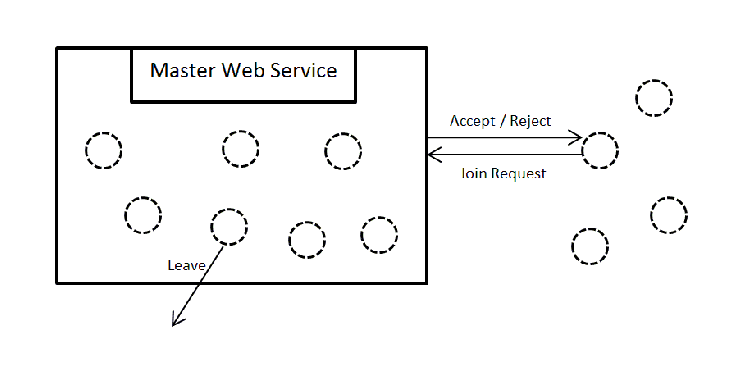
\includegraphics[width=3in]{s1.eps}`
\caption{Web Services and A Grand Community}
\label{fig_sim1}
\end{figure}

The membership decision is made based on throughput and \emph{QoS}
of the considered web service. The goal is to have quality web
services in the community so it stays stable and no other web
services would have incentives to deviate and leave the coalition
$C$. Therefore, a basic method would be to check the core of the
coalition $C$ considering all the current community members (all
web services already residing within the community) and the new
web service. This algorithm uses the \emph{Shapley value}
distribution method as described in Equation \ref{eq:shapley} to
distribute the gain of $v(C)$ among all the members and then
checks if the \emph{Shapley value} payoff vector for this
community having the characteristic function $v(C)$ is in the
\emph{core}. In the \emph{Shapley value} payoff vector, the payoff
for each web service $ws_i$ is calculated based on its marginal
contribution $v(C \cup {i}) - v(C)$ over all the possible
different permutations in which the coalition can be formed, which
makes the payoff distribution fair. Because of going through all
the possible permutations of subsets of $N$, the nature of the
\emph{Shapley value} is combinatorial, which makes it impractical
to use as the size of our coalitions grows. However, it is proven
that in convex games, the \emph{Shapley value} lies in the core
\cite{DBLP:conf/ijcai/GrecoMPS11, myerson1991game}. Thus, if the
\emph{Core} is non-empty, the payoff vector is a member of the
\emph{Core}. The following proposition is important to make our
algorithm tractable.
% so in our algorithm we check the core membership of this payoff vector.

%\ref{eq:convex}.

\newtheorem{theorem}{Proposition}
%\begin{theorem}[Einstein-Podolsky-Rosenberg]
\begin{theorem}\label{proposition1}
A game with a characteristic function $v$
is convex if and only if for all $S$, $T$, and $i$ where $S
\subseteq T \subseteq N \backslash \left\{i\right\}, \forall i \in
N$,
%For $\forall S \subseteq T \subseteq N \backslash \left\{i\right\}, \forall i \in N$ we have:
\begin{equation}\label{eq:convex_snow}
v(S \cup \left\{i\right\}) - v(S) \leq v (T \cup \left\{i\right\}) - v(T)
\end{equation}
\end{theorem}

%\begin{Proposition}\label{proposition} A game with a characteristic function $v$
%is convex if and only if for all $S$, $T$, and $i$ where $S
%\subseteq T \subseteq N \backslash \left\{i\right\}, \forall i \in
%N$,
%For $\forall S \subseteq T \subseteq N \backslash \left\{i\right\}, \forall i \in N$ we have:
%\begin{equation}\label{eq:convex_snow}
%v(S \cup \left\{i\right\}) - v(S) \leq v (T \cup \left\{i\right\}) - v(T)
%\end{equation}
%\end{Proposition}

\begin{proof} 
We first prove the ``only if'' direction:
%\\$~~~~$\textbf{1}. ``only if'' direction:\\
\\$~~~~$\ \textbf{1}. ``only if'' direction:\\
%\setlength{\abovedisplayshortskip}{2pt}
Assume:\\
\vspace{-0.5cm}
\begin{gather*}\label{convexsnowproof}
v(S \cup \left\{i\right\}) - v(S) \leq v (T \cup \left\{i\right\})
- v(T)
\\
\rightarrow v(S \cup \left\{i\right\}) + v(T) \leq v (T \cup \left\{i\right\}) + v(S)
\end{gather*}

Considering $S \subseteq T$:
\setlength{\abovedisplayshortskip}{2pt}
\begin{gather*}
S \cup \left\{i\right\} = (S \cup \left\{i\right\}) \cup T
\\
T = (S \cup \left\{i\right\}) \cap T
\end{gather*}

By setting $A = S \cup \left\{i\right\}$ and $B = T$ we have:
\setlength{\abovedisplayshortskip}{2pt}
\begin{gather*}
v(S \cup \left\{i\right\}) + v(T) \leq v (T \cup \left\{i\right\}) + v(S)
\\
\rightarrow v(S \cup \left\{i\right\}) + v(T) \leq 
\\
v((S \cup \left\{i\right\}) \cup T) + v((S \cup \left\{i\right\}) \cap T)
\\
\rightarrow v(A) + v(B) \leq v(A \cup B) + v(A \cap B)
\end{gather*}
Consequently, the game is convex.

\textbf{2}. ``if'' direction:\\
Assume the game is convex. Thus, for all $A, B \subset N$, we
have: \setlength{\abovedisplayshortskip}{2pt}
\begin{gather*}
v(A) - v(A \cap B) \leq v(A \cup B) - v(B)
\end{gather*}

By setting $S \cup \left\{i\right\} = A$ and $T = B$ where $S \subseteq T$:
\setlength{\abovedisplayshortskip}{2pt}
\begin{gather*}
v(S \cup \left\{i\right\}) - v((S \cup \left\{i\right\}) \cap T) \leq v(T \cup (S \cup \left\{i\right\})) - v(T)
\\
\rightarrow v(S \cup \left\{i\right\}) - v(S) \leq v(T \cup \left\{i\right\}) - v(T)
\end{gather*}

\end{proof}


Thus, in order to keep the characteristic function convex, new web
services should have more marginal contribution as the coalition
size grows.

Our algorithm works as follows. We have an established community
with a master and some member web services already residing in the
community. A web service would send a join request to the
community. The ideal solution would be analyzing the \emph{core}
or \emph{$\epsilon$-core} stability of the group having this new
member. As the normal core membership algorithm is computationally
intractable, we exploit Proposition \ref{proposition1} and Equation
\ref{eq:convex_snow} to check the convexity of our game having
characteristic function where the new member is added. In the
equation, we set $C$ to be our community members $(C)$ before
having the new web service. We assign ${i}$ to the new web
service, and then verify the equation for $S$, setting $ S = T /
W1 $ where $W1$ is the set of all possible subsets of the set $N$
having the size $1$. We can relax the equation a bit by adding a
constant $\epsilon$ to the left side of the equation. We call this
method \emph{Depth-1 Convex-Checker} algorithm. If the equation is
satisfied for all $W1$, we let the new web service join our
community, since the web service will contribute positively enough
to make our new community stable. Since only subsets of size $1$
are checked, the following Proposition holds.

\begin{theorem}\label{complexity1}
\emph{The run time complexity of Depth-1 Convex-Checker algorithm is
$O(n)$.}
\end{theorem}

By this result, we obtain a significant reduction from $O(2^n)$,
which is the complexity of checking all possible subsets of $N$.
In our second method, we use the same algorithm, but this time we
set $W2$ to be the set of all possible subsets of size two and one
of the community $C$. We call this method \emph{Depth-2
Convex-Checker} and its run time complexity is still
linear:

\begin{theorem}\label{complexity2}
\emph{The run time complexity of Depth-2 Convex-Checker algorithm is
$O(n^2)$.}
\end{theorem}

It is possible to develop an anytime algorithm by continuing the
verification of this condition against all subsets of size $3$,
$4$, etc. until the algorithm gets interrupted.

\subsection {Web Services and Many Communities}

In this scenario, we consider multiple communities managed by
multiple master web services, each of which is providing
independent request pools (see Figure \ref{fig_sim2}). Identical
to the first scenario, master web services form coalitions with
web services. We use coalition structure formation methods to
partition web services into non-empty disjoint coalition
structures. As mentioned in Section \ref{sec:coalition}, the used
algorithms \cite{Sandholm1999209,
DBLP:conf/ijcai/GrecoMPS11,DBLP:conf/ijcai/RahwanMJ11} try to
solve key fundamental problems of what coalitions to form, and how
to divide the payoffs among the collaborators.

\begin{figure}[!t]
\centering
\includegraphics[width=3in]{s2.eps}
\caption{Web Services and Many Communities}
\label{fig_sim2}
\end{figure}

In coalition-formation games, formation of the coalitions is the
most important aspect. The solutions focus on maximizing the
social welfare. For any coalition structure $\pi$, let
$v_{cs}(\pi)$ denote the total worth $\sum_{C \in \pi}{v(C)}$,
which represents the \emph{social welfare}. The solution concepts
in this area deal with finding the maximum value for the social
welfare over all the possible coalition structures $\pi$. There
are $centralized$ algorithms for this end, but these approaches
are generally NP-complete. The reason is that the number of all
possible partitions of the set $N$ grows exponentially with the
number of players in $N$, and the centralized algorithms need to
iterate through all these partitions.
%These algorithms \cite{DBLP:conf/ijcai/GrecoMPS11, DBLP:conf/ijcai/RahwanMJ11, RePEc:wpa:wuwpga:0110001} are centralized algorithms, where all the complexity. However these algorithms are more intractable than Core stable solutions and practical with some constraints in practice\cite{RePEc:wpa:wuwpga:0110001}.
In our model, we propose using a distributed algorithm where each
community master and web service can be a decision maker and
decide for its own good. The aim is to find less complex and
distributed algorithms for forming web services
coalitions\cite{DBLP:journals/igtr/AptW09,Dieckmann02dynamiccoalition,ray2007game}.
The distributed merge-and-split algorithm in
\cite{DBLP:journals/igtr/AptW09} suits our application very well.
It keeps splitting and merging coalitions to partitions which are
preferred by all the players inside those coalitions.

This merge-and-split algorithm is designed to be adaptable to
different applications. One major ingredient to use such an
algorithm is a preference relation or well-defined orders proper
for comparing collections of different coalition partitions of the
same set of players. Having two partition sets of players, namely
$P = {P_1,...,P_k}$ and $Q = {Q_1,...Q_l}$, one example would be
to use the social welfare comparison $\sum^k_{i=1}v(P_i) >
\sum^l_{j=1}v(Q_j)$. For our scenario, we use \emph{Pareto order}
comparison, which is an individual-value order appropriate for our
self-interest web services. In the Pareto order, an allocation or
partition $P$ is preferred over another $Q$ if at least one player
improves its payoff in the new allocation and all the other
players still maintain their payoff ($p_i \geq q_i$ with at least
one element $p_i > q_i$).

The valuation function $v(C)$ for this scenario is the same as
\emph{``Web Services and One Community''} scenario. However, in
order to prevent master web services joining the same community,
we set $v(C) = 0$ when $C$ has either none, or more than one
master web service as member.

In this scenario, as new web services are discovered and get ready
to join communities, our algorithm keeps merging and splitting
partitions based on the preference function. The decision to merge
or split is based on the fact that all players must benefit. The
new web services will merge with communities if $all$ the players
are able to improve their individual payoff, and some web services
may split from old communities, if splitting does not decrease the
payoff of any web service of the community. According to
\cite{DBLP:journals/corr/abs-cs-0605132}, this sequence of merging
and splitting will converge to a final partition, where web
services cannot improve their payoff. More details of this
algorithm and analysis of generic solutions on coalition formation
games are described in \cite{DBLP:journals/igtr/AptW09}.


\subsection {Web Services Collaborating Independently}

In this scenario, there is no pre-defined community and web
services are interested in forming new ones to perform better and
share benefits (see Figure \ref{fig_sim3}). Consequently, there is
no master web service providing requests for others, but each web
service comes with its own request load called \emph{market
share}. Communities can be formed because by working together web
services can expect to gain more than working individually. The
worth or value of a coalition of web services is different in this
setting. Let $metrics$ be the set of quality metrics, we average
the values $Q^m_{ws}$ for all quality metrics ($m \in metrics$)
for each web service $ws$, multiply it by a weight reflecting the
importance of each metric for each web service ($w^m_{ws}$) (Note
that $ \sum_{m}{w^m_{ws}} = 1 $). For each web service, we
multiply this weighted average by web service's market share
$(\mu_{ws})$ and the summation over all the web services of the
community to be established would be the characteristic or
valuation function. This function has the property to be
increasing in the market share and QoS.

\begin{equation}
v(C) = \sum_{ws \in C}{ \Big( \frac{\sum_{m \in metrics}{Q^m_{ws}
\times w^m_{ws}}}{|metrics|} \Big) \times \mu_{ws} }
\end{equation}

%$CC^{m}$ is \emph{Collabrative Coefficient} for each QoS metric (non-functional parameter), it determines how web services providing that QoS metric individually will be effected in a coalition environment. If it is more than 1, is means they increase performance by working together and they are \emph{super additive}, otherwise it depicts they would perform better in linear sense if they worked alone.
As there is no pre-defined master web services in this scenario,
we assume that the members of each coalition either dynamically
vote for one, or collaborate and distribute tasks in round robin
or fair fashion. To form stable coalitions, we use the same
merge-and-split algorithm we applied for the \emph{``Web Services
and Many Communities''} scenario.

\begin{figure}[!t]
\centering
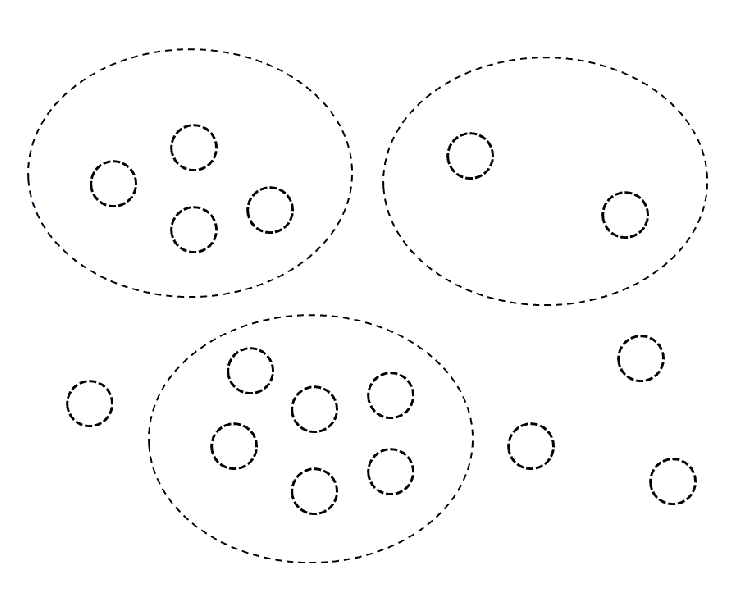
\includegraphics[width=3in]{s3.eps}
\caption{Web Services collaborating independently}
\label{fig_sim3}
\end{figure}

\section{Experimental Results and Analysis}\label{s:resutls}

In this section, we discuss the experiments we performed for our
scenarios to validate the applicability and performance of our
proposed methods in realistic environments. We created a pool of
web services and populated most of their \emph{QoS} parameters
from a real world web service dataset
\cite{DBLP:conf/smc/Al-MasriM09a}. We implemented the simulations
using Java and executed the simulations on an Intel Xeon X3450
machine with 4GBs of memory. For other parameters missing from the
dataset, we used normal random distribution with parameters
estimated using the method of maximum likelihood.

One of the key criteria reflecting the performance of web service
coalitions is the user satisfaction. User satisfaction can be
measured in terms of quality and quantity of requests (or tasks)
successfully answered by the communities. We initiate the
communities with few web services, then let rejecting and
accepting random web services go for a short number of iterations.
After that, we start the request distribution for the communities
and let them allocate requests among member web services.
Thereafter, we measure the average output performance of tasks in
communities following different methods.

\begin{figure}[!t]
\centering
%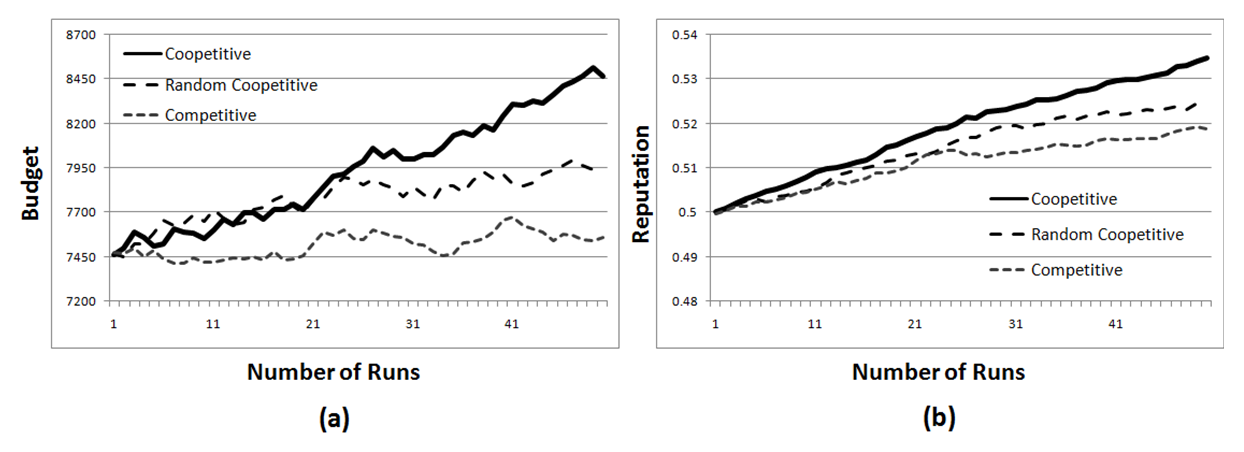
\includegraphics[scale=0.6]{graph1Final+.eps}
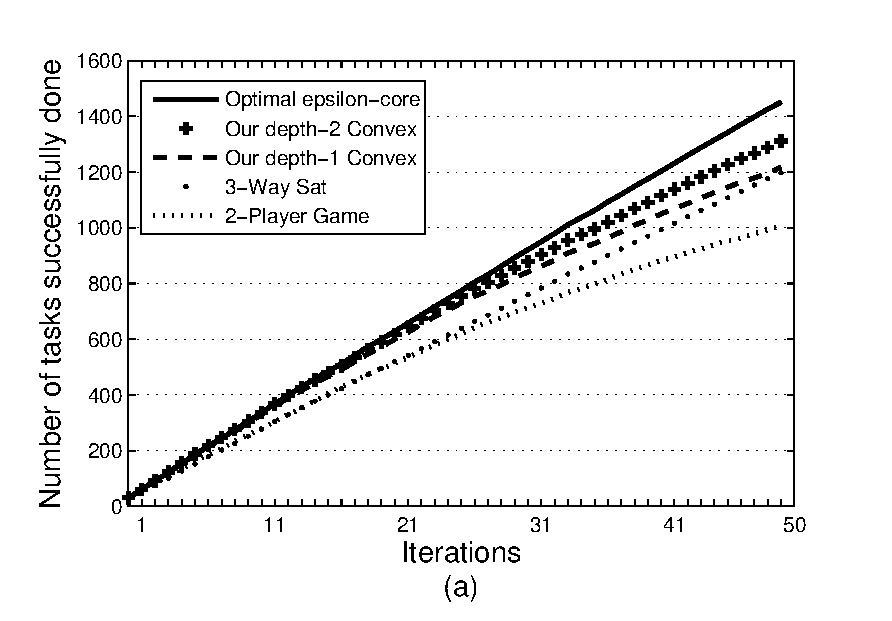
\includegraphics[width=3in]{task_done_opt.eps}
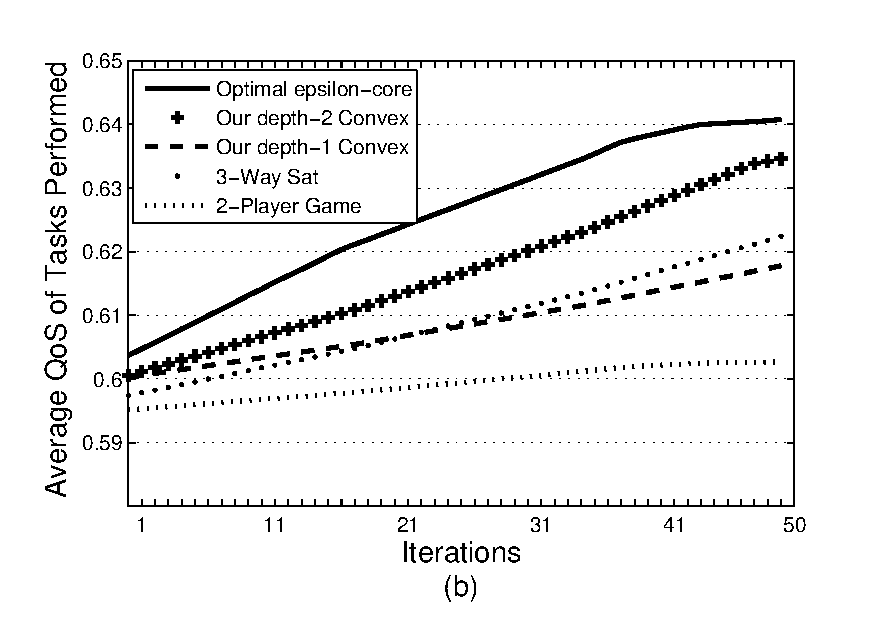
\includegraphics[width=3in]{task_qos_opt.eps}
\caption{Part (a): Cumulative number of requests successfully
done. Part (b): Average QoS of requests performed.}
\label{performanceall}
\end{figure}

Figure \ref{performanceall} depicts the results of optimal
\emph{$\epsilon$-core}, \emph{Depth-1 Convex-Checker},
\emph{Depth-2 Convex-Checker}, \emph{3-Way Satisfaction}
\cite{DBLP:conf/IEEEscc/LimTMB12}, and \emph{2 Player
Non-Cooperative} \cite{DBLP:conf/IEEEscc/KhosravifarABT11} methods
in \emph{one grand community with many web services} scenario. For
\emph{$\epsilon$-core}, we assign $\epsilon$ to 15\% of total
community worth, $\epsilon = 0.15 \times v(C)$, which allows
subsets of the coalition to gain maximum 15\% of $v(C)$. In the
\emph{optimal $\epsilon$-core} method, we capped the coalition
size to 25 web services, since the method is computationally 
intractable and anything more than that would make it
impractical to run in our simulations. In the other methods, there
were no cap on size of the community and we had communities of
size 60 web services at some points. The results show that our
\emph{depth-2 convex checker} method is performing better compared
to the other methods and its performance is close to optimal
\emph{$\epsilon$-core} method. Our \emph{depth-1 convex checker}
and the \emph{3-Way Satisfaction} method, are also performing well.


\begin{figure}[!t]
\centering
%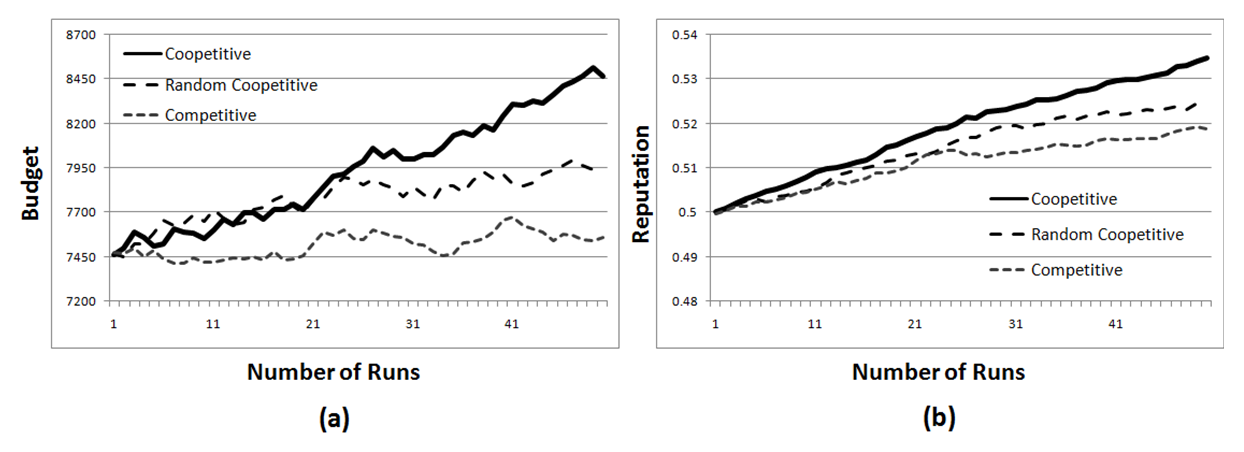
\includegraphics[scale=0.6]{graph1Final+.eps}
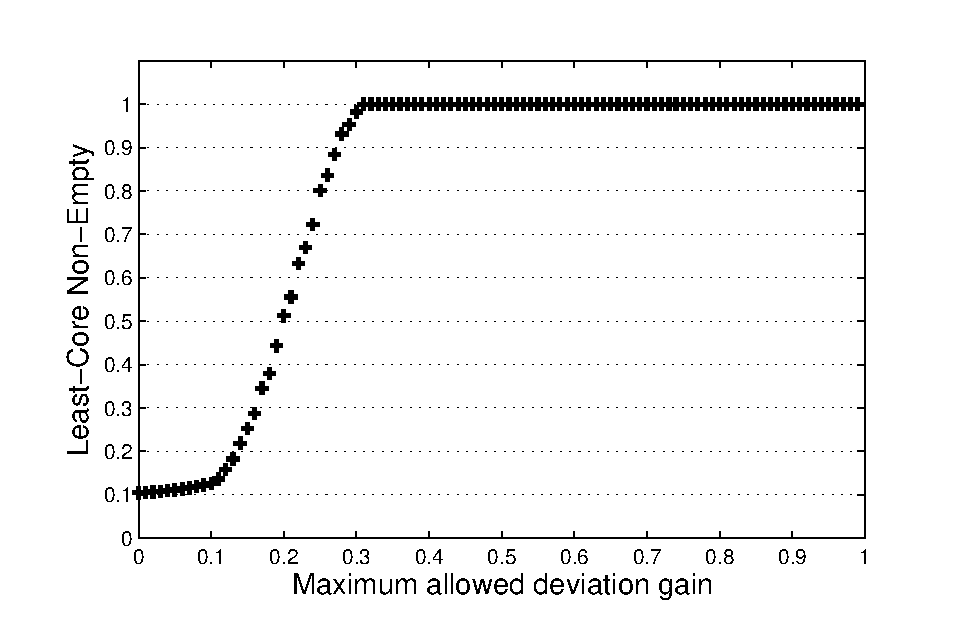
\includegraphics[width=3in]{least_core.eps}
\caption{Analysis of \emph{$\epsilon$-core} set non-emptiness, for different values of $\epsilon$} \label{f_leastcore}
\end{figure}

As mentioned in Section \ref{s:preliminaries}, the concept of
\emph{core}, assumes no coalition of players can gain anything by
deviating, which is a fairly strong requirement, and that is why
the notion of \emph{$\epsilon$-core} was introduced. Least-Core
$e(G)$ of a game $G$, is the minimum amount of $\epsilon$ so that
the core is not empty. We evaluated the non-emptiness of \emph{$\epsilon$-core} set using the
valuation function and a set of web services. We picked random
number of web services from the dataset and formed around 10,000
random coalitions consisting of 3 to 26 web services. We choose 26
as the maximum number of members in our coalition since it
is computationally very complex for larger coalitions to verify whether 
\emph{$\epsilon$-core} set is empty or not. Also instead of considering $\epsilon$ amount of constant deviation in \emph{$\epsilon$-core} definition (Equation \ref{eq:core2}), we similarly defined \emph{relative $\epsilon$-core} concept where no coalition would benefit more than \emph{$\epsilon$ $\times$ v(C)} by deviating. We set $\epsilon$ between 0 and 1 and verify the \emph{relative $\epsilon$-core} set non-emptiness. The results in Figure
\ref{f_leastcore} illustrates that almost 10\% of our random web
service coalitions have non-empty \emph{core} solution and
\emph{$\epsilon$-core} solution is \emph{always} non-empty when we
let agents gain only 30\% more of $v(C)$ by deviating.

One of the properties of coalition structure formation algorithms
in our third scenario is that they partition web services with low
throughput rate so that they usually join coalitions with less
request rate. Since the characteristic function $v(C)$ and the
fair Shapely payoff vector is proportional to web services'
contribution, the web services with small contribution will get
paid much less in communities having web services with high
throughput. On the other hand, according to the valuation function
$v(C)$, web services with high throughput will not contribute well
to communities with low amount of user requests (low market
share). The strong web services are likely to deviate from weak
coalitions, joining a stronger one, which makes the initial
coalition unstable.

\begin{figure}[!t]
\centering
%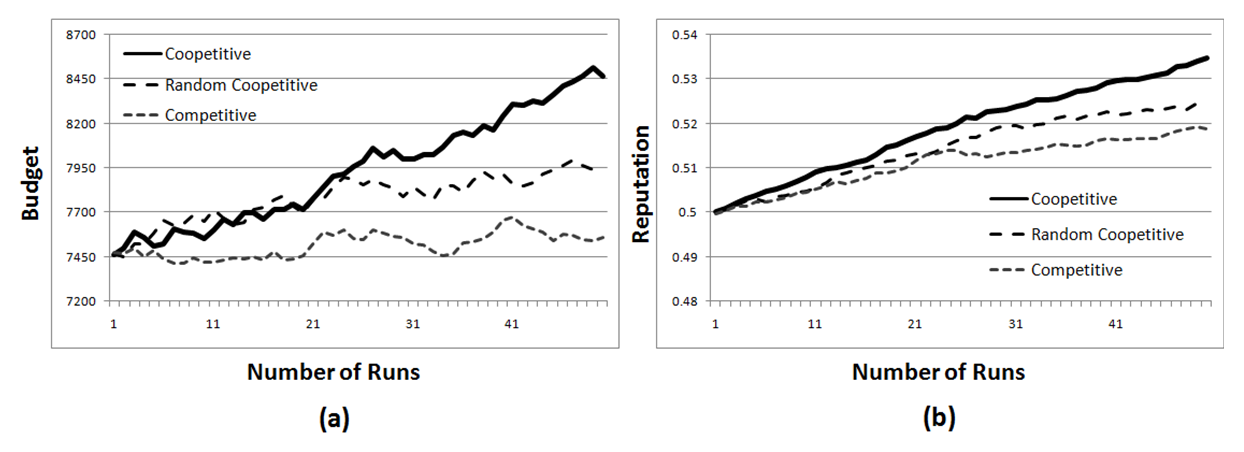
\includegraphics[scale=0.6]{graph1Final+.eps}
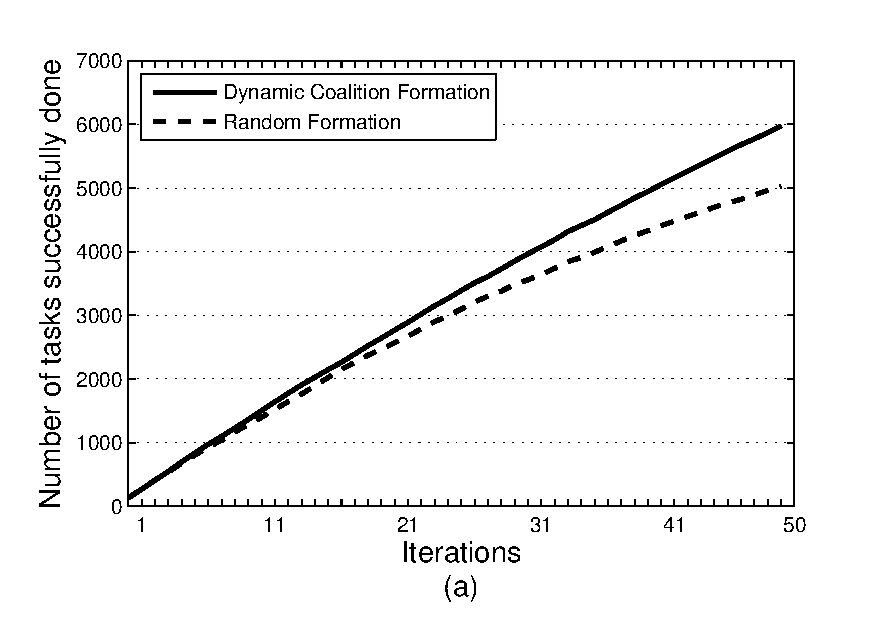
\includegraphics[width=3in]{s2_task_done.eps}
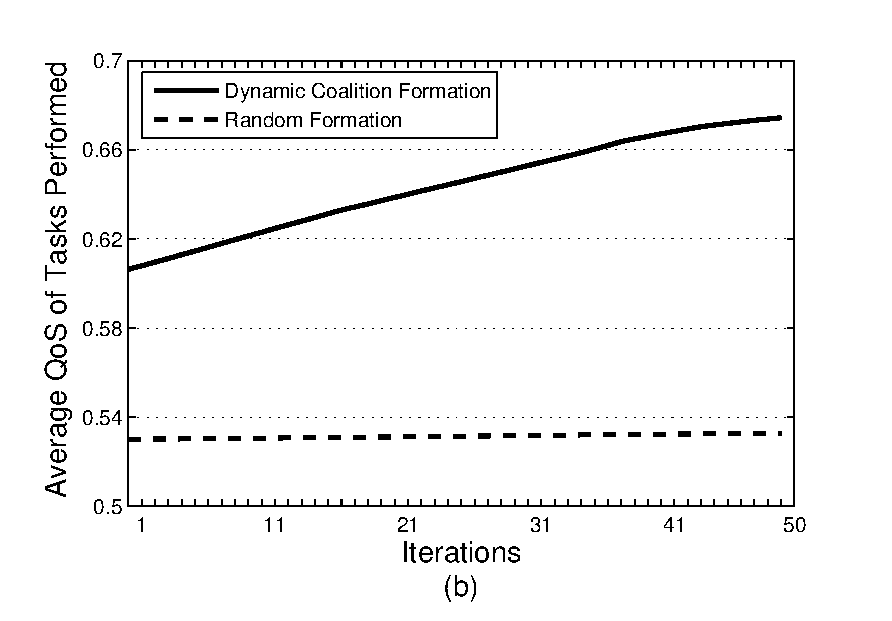
\includegraphics[width=3in]{s2_task_qos.eps}
\caption{Part (a): Cumulative number of tasks succesfully done. Part
(b): Average QoS of tasks performed.} \label{performancemany}
\end{figure}

In Figure \ref{performancemany}, we compare our \emph{Web Services
and many Communities} scenario with a method which ignores QoS
parameters and forms coalitions by allowing web services to join
only if they have enough requests for themselves. In other words,
web services can join a community when the request rate is less
than the throughput of all the member web services. We name this
method \emph{Random Formation} and use it as a benchmark for our
QoS-aware coalition formation process. As the results illustrate,
our method forms better coalitions of web services improving
performance and satisfaction for both web services and coalitions.


\section{Related Work}\label{s:relatedwork}

Game theory provides a rich set of frameworks and mathematical tools for rational agents seeking to maximise their profit and efficiency through choosing best available streteghies in multi-agent enviroments.

%\subsection{Subsection Heading Here}
%Subsection text here.

% needed in second column of first page if using \IEEEpubid
%\IEEEpubidadjcol

%\subsubsection{Subsubsection Heading Here}
%Subsubsection text here.Subsubsection text here.Subsubsection text here.Subsubsection text here.Subsubsection text here.Subsubsection text here.Subsubsection text here.Subsubsection %text here.Subsubsection text here.Subsubsection text here.Subsubsection text here.Subsubsection text here.Subsubsection text here.
%Subsubsection text here.Subsubsection text here.Subsubsection text here.

%Subsubsection text here.Subsubsection text here.Subsubsection text here.Subsubsection text here.Subsubsection text here.Subsubsection text here.Subsubsection text here.Subsubsection %text here.Subsubsection text here.Subsubsection text here.Subsubsection text here.Subsubsection text here.Subsubsection text here.Subsubsection text here.


% An example of a floating figure using the graphicx package.
% Note that \label must occur AFTER (or within) \caption.
% For figures, \caption should occur after the \includegraphics.
% Note that IEEEtran v1.7 and later has special internal code that
% is designed to preserve the operation of \label within \caption
% even when the captionsoff option is in effect. However, because
% of issues like this, it may be the safest practice to put all your
% \label just after \caption rather than within \caption{}.
%
% Reminder: the "draftcls" or "draftclsnofoot", not "draft", class
% option should be used if it is desired that the figures are to be
% displayed while in draft mode.
%
%\begin{figure}[!t]
%\centering
%\includegraphics[width=2.5in]{myfigure}
% where an .eps filename suffix will be assumed under latex, 
% and a .pdf suffix will be assumed for pdflatex; or what has been declared
% via \DeclareGraphicsExtensions.
%\caption{Simulation Results}
%\label{fig_sim}
%\end{figure}

% Note that IEEE CS typically puts floats only at the top, even when this
% results in a large percentage of a column being occupied by floats.
% However, the Computer Society has been known to put floats at the bottom.


% An example of a double column floating figure using two subfigures.
% (The subfig.sty package must be loaded for this to work.)
% The subfigure \label commands are set within each subfloat command, the
% \label for the overall figure must come after \caption.
% \hfil must be used as a separator to get equal spacing.
% The subfigure.sty package works much the same way, except \subfigure is
% used instead of \subfloat.
%
%\begin{figure*}[!t]
%\centerline{\subfloat[Case I]\includegraphics[width=2.5in]{subfigcase1}%
%\label{fig_first_case}}
%\hfil
%\subfloat[Case II]{\includegraphics[width=2.5in]{subfigcase2}%
%\label{fig_second_case}}}
%\caption{Simulation results}
%\label{fig_sim}
%\end{figure*}
%
% Note that often IEEE CS papers with subfigures do not employ subfigure
% captions (using the optional argument to \subfloat), but instead will
% reference/describe all of them (a), (b), etc., within the main caption.


% An example of a floating table. Note that, for IEEE style tables, the 
% \caption command should come BEFORE the table. Table text will default to
% \footnotesize as IEEE normally uses this smaller font for tables.
% The \label must come after \caption as always.
%
%\begin{table}[!t]
%% increase table row spacing, adjust to taste
%\renewcommand{\arraystretch}{1.3}
% if using array.sty, it might be a good idea to tweak the value of
% \extrarowheight as needed to properly center the text within the cells
%\caption{An Example of a Table}
%\label{table_example}
%\centering
%% Some packages, such as MDW tools, offer better commands for making tables
%% than the plain LaTeX2e tabular which is used here.
%\begin{tabular}{|c||c|}
%\hline
%One & Two\\
%\hline
%Three & Four\\
%\hline
%\end{tabular}
%\end{table}


% Note that IEEE does not put floats in the very first column - or typically
% anywhere on the first page for that matter. Also, in-text middle ("here")
% positioning is not used. Most IEEE journals use top floats exclusively.
% However, Computer Society journals sometimes do use bottom floats - bear
% this in mind when choosing appropriate optional arguments for the
% figure/table environments.
% Note that, LaTeX2e, unlike IEEE journals, places footnotes above bottom
% floats. This can be corrected via the \fnbelowfloat command of the
% stfloats package.



\section{Conclusion}\label{s:conclusion}

In this paper, we proposed a cooperative game theory-based model
for the aggregation of web services within communities. The goal
of our services is to maximize efficiency by collaborating and
forming stable coalitions. Our method considers stability and
fairness for all web services within a community and offers an
applicable mechanism for membership requests and selection of web
services. The ultimate goal is to increase revenue by improving
user satisfaction, which comes from the ability to perform more
tasks with high quality. Simulation results show that our,
polynomial in complexity, approximation algorithms provide web
services and community owners with applicable and near-optimal
decision making mechanisms.

As future work, we would like to perform more analytical and
theoretical analysis on the convexity condition and also minimal $\epsilon$ values in \emph{$\epsilon$-core} solution concepts based on the
characteristic function in web service applications. From web service perspective, the
work can be extended to consider web service compositions where a
group of web services having different set of skills cooperate to
perform composite tasks. Also bargaining theory from cooperating
game theory concepts can be used to help web services resolve the
instability and unfairness issues by side payments.





% if have a single appendix:
%\appendix[Proof of the Zonklar Equations]
% or
%\appendix  % for no appendix heading
% do not use \section anymore after \appendix, only \section*
% is possibly needed

% use appendices with more than one appendix
% then use \section to start each appendix
% you must declare a \section before using any
% \subsection or using \label (\appendices by itself
% starts a section numbered zero.)
%


%\appendices
%\section{Proof of the First Zonklar Equation}
%Appendix one text goes here.

% you can choose not to have a title for an appendix
% if you want by leaving the argument blank
%\section{}
%Appendix two text goes here.Appendix two text goes here.Appendix two text goes here.Appendix two text goes here.Appendix two text goes here.Appendix two text goes here.Appendix two text goes here.Appendix two text goes here.Appendix two text goes here.Appendix two text goes here.Appendix two text goes here.Appendix two text goes here.Appendix two text goes here.Appendix two text goes here.Appendix two text goes here.Appendix two text goes here.Appendix two text goes here.Appendix two text goes here.Appendix two text goes here.Appendix two text goes here.Appendix two text goes here.Appendix two text goes here.Appendix two text goes here.Appendix two text goes here.Appendix two text goes here.


% use section* for acknowledgement
\ifCLASSOPTIONcompsoc
  % The Computer Society usually uses the plural form
  \section*{Acknowledgments}
\else
  % regular IEEE prefers the singular form
  \section*{Acknowledgment}
\fi


The authors would like to thank...The authors would like to thank...The authors would like to thank...The authors would like to thank...The authors would like to thank...The authors would like to thank...The authors would like to thank...The authors would like to thank...The authors would like to thank...The authors would like to thank...The authors would like to thank...The authors would like to thank...The authors would like to thank...


% Can use something like this to put references on a page
% by themselves when using endfloat and the captionsoff option.
\ifCLASSOPTIONcaptionsoff
  \newpage
\fi



% trigger a \newpage just before the given reference
% number - used to balance the columns on the last page
% adjust value as needed - may need to be readjusted if
% the document is modified later
%\IEEEtriggeratref{8}
% The "triggered" command can be changed if desired:
%\IEEEtriggercmd{\enlargethispage{-5in}}

% references section

\bibliographystyle{IEEEtran}
\bibliography{Ehsan}

% can use a bibliography generated by BibTeX as a .bbl file
% BibTeX documentation can be easily obtained at:
% http://www.ctan.org/tex-archive/biblio/bibtex/contrib/doc/
% The IEEEtran BibTeX style support page is at:
% http://www.michaelshell.org/tex/ieeetran/bibtex/
%\bibliographystyle{IEEEtran}
% argument is your BibTeX string definitions and bibliography database(s)
%\bibliography{IEEEabrv,../bib/paper}
%
% <OR> manually copy in the resultant .bbl file
% set second argument of \begin to the number of references
% (used to reserve space for the reference number labels box)
%\begin{thebibliography}{1}

%\bibitem{IEEEhowto:kopka}
%This is an example of a book reference
%H. Kopka and P.W. Daly, \emph{A Guide to {\LaTeX}}, third ed. Harlow, U.K.: Addison-Wesley, 1999.


%This is an example of a Transactions article reference
%D.S. Coming and O.G. Staadt, "Velocity-Aligned Discrete Oriented Polytopes for Dynamic Collision Detection," IEEE Trans. Visualization and Computer Graphics, vol.�14,� no.�1,� pp. 1-12,� Jan/Feb� 2008, doi:10.1109/TVCG.2007.70405.

%This is an example of a article from a conference proceeding
%H. Goto, Y. Hasegawa, and M. Tanaka, "Efficient Scheduling Focusing on the Duality of MPL Representation," Proc. IEEE Symp. Computational Intelligence in Scheduling (SCIS '07), pp. 57-64, Apr. 2007, doi:10.1109/SCIS.2007.367670.

%This is an example of a PrePrint reference
%J.M.P. Martinez, R.B. Llavori, M.J.A. Cabo, and T.B. Pedersen, "Integrating Data Warehouses with Web Data: A Survey," IEEE Trans. Knowledge and Data Eng., preprint, 21 Dec. 2007, doi:10.1109/TKDE.2007.190746.

%Again, see the IEEEtrans_HOWTO.pdf for several more bibliographical examples. Also, more style examples
%can be seen at http://www.computer.org/author/style/transref.htm
%\end{thebibliography}

% biography section
% 
% If you have an EPS/PDF photo (graphicx package needed) extra braces are
% needed around the contents of the optional argument to biography to prevent
% the LaTeX parser from getting confused when it sees the complicated
% \includegraphics command within an optional argument. (You could create
% your own custom macro containing the \includegraphics command to make things
% simpler here.)
%\begin{biography}[{\includegraphics[width=1in,height=1.25in,clip,keepaspectratio]{mshell}}]{Michael Shell}
% or if you just want to reserve a space for a photo:

\begin{IEEEbiography}{Michael Shell}
Biography text here.
\end{IEEEbiography}

% if you will not have a photo at all:
\begin{IEEEbiographynophoto}{John Doe}
Biography text here.Biography text here.Biography text here.Biography text here.Biography text here.Biography text here.Biography text here.Biography text here.Biography text here.Biography text here.Biography text here.Biography text here.Biography text here.Biography text here.Biography text here.Biography text here.Biography text here.Biography text here.Biography text here.Biography text here.Biography text here.Biography text here.Biography text here.Biography text here.Biography text here.Biography text here.Biography text here.Biography text here.Biography text here.Biography text here.Biography text here.Biography text here.
\end{IEEEbiographynophoto}

% insert where needed to balance the two columns on the last page with
% biographies
%\newpage

\begin{IEEEbiographynophoto}{Jane Doe}
Biography text here.Biography text here.Biography text here.Biography text here.Biography text here.Biography text here.Biography text here.Biography text here.Biography text here.Biography text here.Biography text here.Biography text here.Biography text here.Biography text here.Biography text here.Biography text here.Biography text here.Biography text here.Biography text here.Biography text here.Biography text here.Biography text here.Biography text here.Biography text here.Biography text here.Biography text here.Biography text here.Biography text here.
\end{IEEEbiographynophoto}

% You can push biographies down or up by placing
% a \vfill before or after them. The appropriate
% use of \vfill depends on what kind of text is
% on the last page and whether or not the columns
% are being equalized.

%\vfill

% Can be used to pull up biographies so that the bottom of the last one
% is flush with the other column.
%\enlargethispage{-5in}



% that's all folks
\end{document}



